\subsection{Generalisations}
\label{ssec:relating-variations}

The results of the previous subsections carry across to non-binary, fixed
arity synchronisations, in a straightforward way.  For a $k$-ary
synchronisation between distinct operations |op|\s1, \ldots, |op|$_k$, the
corresponding two-step linearisation specification object has $2k-1$
operations, |op|\s1, \ldots, |op|$_k$, $\overline{\sm{op}}_1$, \ldots,
$\overline{\sm{op}}_{k-1}$.  The definition of two-step linearisation is then
the obvious adaptation of the binary case: each operation |op|\s{i} of the
synchronisation object is linearised by the composition of |op|\s{i} and
$\overline{\op}_i$ of the specification object, for $i = 1, \ldots, k-1$.

%% Each of the first $k - 1$ |op| operations takes a thread identity as a
%% parameter.

The construction of the previous subsection is easily adapted to the case of
$k$-way synchronisations for $k > 2$.  The specification object encodes an
automaton with $k$ states.  The figure below gives the automaton in the case
$k = 4$.
%
\begin{center}
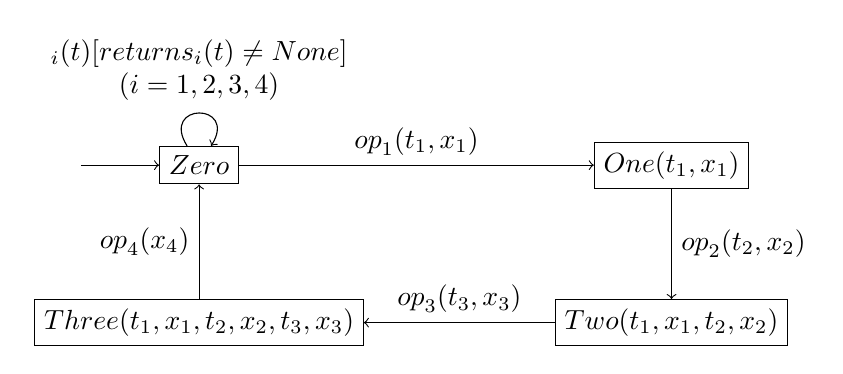
\begin{tikzpicture}[xscale = 1]
\draw (0,0) node[draw] (zero) {$\sm{Zero}$};
\draw[->] (zero) ++ (-1.5, 0) -- (zero);
\draw[->] (zero) .. controls ++(-0.5,+0.8) and ++(0.5,0.8) .. 
  node[above]{
    $\begin{array}{c}
      \overline{\op}_i(t) [\sm{returns}_i(t) \ne \sm{None}] \\ (i = 1,2,3,4)
    \end{array}$}
  %% $\overline{\op}_1,\, \overline{\op}_2,\, 
  %%  \overline{\op}_3,\, \overline{\op}_4$}
  (zero);
%
\draw (zero)++(6,0) node[draw] (one) {$\sm{One}(\sm{t}_1, \sm{x}_1)$};
\draw[->] (zero)  -- node[above] {$\sm{op}_1(\sm{t}_1, \sm{x}_1)$} (one); 
%
\draw (one)++(0, -2) node[draw] (two) 
  {$\sm{Two}(\sm{t}_1, \sm{x}_1, \sm{t}_2, \sm{x}_2)$};
\draw[->] (one)  -- node[right] {$\sm{op}_2(\sm{t}_2, \sm{x}_2)$} (two); 
%
\draw (two)++(-6, 0) node[draw] (three) 
  {$\sm{Three}(\sm{t}_1, \sm{x}_1, \sm{t}_2, \sm{x}_2, \sm{t}_3, \sm{x}_3)$};
\draw[->] (two)  -- node[above] {$\sm{op}_3(\sm{t}_3, \sm{x}_3)$} (three); 
%
%% \draw (three)++(0,-2) node[draw] (threeX) 
%%   {$\sm{ThreeX}(\sm{y}_1, \sm{y}_2, \sm{y}_3)$};
\draw[->] (three)  -- node[left] {$\sm{op}_4(\sm{x}_4)$} (zero); 
%
%% \draw (threeX)++(-4,0) node[draw] (twoX) {$\sm{TwoX}(\sm{y}_1, \sm{y}_2)$};
%% \draw[->] (threeX)  -- node[above] {$\overline{\sm{op}}_3()$} (twoX); 
%% %
%% \draw (twoX)++(-3.5,0) node[draw] (oneX) {$\sm{OneX}(\sm{y}_1)$};
%% \draw[->] (twoX)  -- node[above] {$\overline{\sm{op}}_2()$} (oneX);
%% \draw [->] (oneX)  -- node[below] {$\overline{\sm{op}}_1()$} (zero);
\end{tikzpicture}
\end{center}
%
The final |op| operation, |op|\s4 in the above figure, applies the |sync|
method of the synchronisation specification object to the parameters $\sm x_1,
\ldots, \sm x_k$ to obtain the results $\sm y_1, \ldots, \sm y_k$; it stores
the first $k-1$ in appropriate |returns|\s{i} arrays, and returns $\sm y_k$
itself.  In the case $k=4$, it has definition:
%
\begin{scala}
  def op£\s4£(x£\s4£: A£\s4£): B£\s4£ = {
    require(state.isInstanceOf[Three]); val Three(t£\s1£, x£\s1£, t£\s2£, x£\s2£, t£\s3£, x£\s3£) = state
    val (y£\s1£, y£\s2£, y£\s3£, y£\s4£) = SyncSpec.sync(x£\s1£, x£\s2£, x£\s3£, x£\s4£) 
    returns£\s1£(t£\s1£) = Some(y£\s1£); returns£\s2£(t£\s2£) = Some(y£\s2£); returns£\s3£(t£\s3£) = Some(y£\s3£)
    state = Zero; y£\s4£
  }
\end{scala}
%
Each $\overline{\sm{op}}_i$ operation retrieves the result from the
corresponding |returns|\s{i} array.

%%%%%%%%%%%%%%%%%%%%%%%%%%%%%%%%%%%%%%%%%%%%%%%%%% Homogeneous

We now consider the homogeneous case.  For simplicity, we describe the binary
case; synchronisations of more than two invocations are handled similarly.
Suppose we have a synchronisation object with a single operation 
\SCALA{def op(x: A): B}.
All invocations of~|op| have to be treated similarly, so we associate
\emph{each} with two operations |op| and $\overline{\sm{op}}$ of the
specification object.  The specification object is below, and encodes the
automaton on the right.
%% %
%% \begin{center}
%% \begin{tikzpicture}[>= angle 60, xscale = 0.9, yscale = 0.44]
%% \draw (0,0) node[draw] (zero) {$\sm{Zero}$};
%% \draw[->] (zero) ++ (-1.5, 0) -- (zero);
%% %
%% \draw (4,0) node[draw] (one) {$\sm{One}(\sm t_1, \sm{x}_1)$};
%% \draw[->] (zero) .. controls ++(1.75,0.6) .. 
%%   node[above] {$\sm{op}(\sm t_1, \sm{x}_1)$} (one); 
%% %
%% \draw[<-] (zero) .. controls ++(1.75,-0.6) .. 
%%   node[below] {$\sm{op}(\sm t_2, \sm x_2)$} (one);
%% \end{tikzpicture}
%% \end{center}
%
The second invocation of |op| in any synchronisation (from the |One| state of the
automaton) writes the results of the invocation into the |returns| array.
Each invocation of $\overline{\sm{op}}$ returns the stored value.

\begin{trivlist}
\item[]
\begin{minipage}{92mm}
\begin{scala}
class TwoStepLinSpec{
  private var state: State = Zero
  private val returns = new Array[Option[B£\s1£]](NumThreads)
  for(t <- 0 until NumThreads) returns(t) = None
  def op(t: ThreadID, x: A): Unit = {
    require(returns(t) == None)
    state match{
      case Zero => state = One(t, x)
      case One(t£\s1£, x£\s1£) => 
        val (y£\s1£, y£\s2£) = SyncSpec.sync(x£\s1£, x) 
        returns(t£\s1£) = Some(y£\s1£); returns(t) = Some(y£\s2£); state = Zero
    }
  }
  def £$\overline{\sm{op}}$£(t: ThreadID): B = {
    require(state.isInstanceOf[Zero] && returns(t).isInstanceOf[Some])
    val Some(y) = returns(t); returns(t) = None; y
  }
}
\end{scala}
\end{minipage}
\hfill 
%
\begin{minipage}{37.8mm}
\begin{tikzpicture}[>= angle 60, xscale = 0.9, yscale = 0.44]
\draw (0,0) node[draw] (zero) {$\sm{Zero}$};
\draw[->] (zero) ++ (-1.5, 0) -- (zero);
\loopAbove(zero){$\begin{array}{c}
  \overline\op(\sm t) \\ {[\sm{returns(t)} \ne \sm{None}]}
  \end{array}$}
%
\draw (0,-4) node[draw] (one) {$\sm{One}(\sm t_1, \sm{x}_1)$};
\draw[->] (zero) .. controls ++(0.3,-2) .. 
  node[right] {$\sm{op}(\sm t_1, \sm{x}_1)$} (one); 
%
\draw[->] (one) .. controls ++(-0.3,2) .. 
  node[left] {$\sm{op}(\sm t_2, \sm x_2)$} (zero);
\end{tikzpicture}%
\vspace{40mm}
\end{minipage}%
\end{trivlist}


%%%%%%%%%%%%%%%%%%%%%%%%%%%%%%%%%%%%%%%%%%%%%%%%%%%%%%% Mixed arity


Recall that some operations may have mixed modes of synchronisations:
different invocations may have synchronisations with different arities.  For
example, in a timeout channel, an invocation of the |send| and |receive|
operations may synchronise with an invocation of the other operation, or may
timeout corresponding to a unary synchronisation.
%
%% We illustrate how to test for synchronisation linearisation of objects with
%% mixed modes of synchronisation via an example.

Figure~\ref{fig:two-step-timeout-chan} gives the automaton for a timeout
channel, where we treat $\send$ as corresponding to $\op_1$ (we omit concrete
code in the interests of brevity).  The automaton is similar to that for a
standard channel.  The |receive| operation can happen from either state: if it
happens from the |One| state, then a synchronisation has occurred and the
invocation returns a value of the form |Some(x)|; but if it happens from the
|Zero| state, there has been no corresponding |send|, and so the invocation
returns~|None|, indicating a timeout.  Likewise, the $\overline{\send}$
operation can happen from either state; if it happens from the |Zero| state,
then a synchronisation has occurred and the invocation returns |true|; but if
it happens from the |One| state, there has been no corresponding |receive|,
and so the invocation returns~|false|, indicating a timeout.

\begin{figure}
\begin{center}
\begin{tikzpicture}[>= angle 60, xscale = 0.9, yscale = 0.44]
\draw (0,0) node[draw] (zero) {$\sm{Zero}$};
\draw[->] (zero) ++ (-1.5, 0) -- (zero);
% self-loop on Zero
\loopAbove(zero){$\begin{array}{@{}c@{}}
      \receive()\::\sm{None}, \\ 
      \overline{\send}(\sm t)\::\sm{true} [\sm{returns(t)} \ne \sm{None}]
    \end{array}$}
%%%%%% One
\draw (0,-5) node[draw] (one) {$\sm{One}(\sm t, \sm{x})$};
\draw[->] (zero) .. controls ++(0.3,-2.5) .. 
  node[right] {$\send(\sm t, \sm{x})$} (one); 
\draw[->] (one) .. controls ++(-0.3,2.5) .. 
  node[left] {$\begin{array}[t]{r@{}}
   \receive()\::\sm{Some(x)}, \\ \overline{\send}(\sm t)\::\sm{false}
    \end{array}$} (zero);
\end{tikzpicture}
\end{center}
\caption{Automaton for capturing two-step linearisation for a timeout
  channel.}
\label{fig:two-step-timeout-chan}
\end{figure}

%% It is interesting to ask whether we can optimise the above construction, using
%% just a single transition in the case of a failed send.  It turns out that we
%% cannot.  To do so we require \emph{two} |send| transitions from |Zero|,
%% corresponding to successful and unsuccessful cases (leading to |One| and
%% |Zero| states, respectively).  This would make the automaton nondeterministic,
%% contrary to our assumptions.



%%%%%%%%%%%%%%%%%%%%%%%%%%%%%%%%%%%%%%%%%%%%%%%%%%%%%%% Stateful

We now consider stateful specification objects.  In general, we can simply
augment the |Zero| and |One| states of the automaton to include the state of
the specification object.  Note that different transitions may be available
based upon that state.  
%% For example, with a closeable channel, we could include a boolean field in
%% the automaton states, indicating whether the channel is closed.
However, it can be clearer and simpler to introduce
different named states into the automaton.

%% , as in
%% Figure~\ref{fig:two-step-closeable-chan}, where the automaton has an
%% additional state, |Closed|, corresponding to the channel being closed.  

%% It is also possible to capture operations with mixed modes of synchronisations
%% where the arity of each invocation depends upon the state of the
%% synchronisation object.  

Figure~\ref{fig:two-step-closeable-chan} gives the specification automaton for
a closeable channel.  The automaton has an additional state, |Closed|,
corresponding to the channel being closed.  All invocations are unary
synchronisations in this state.  This automaton represents a simplification
over the general approach discussed above: we do not need two separate states
after closing.  Note that a $\overline{\send}(\sm t)$ transition from the
|Closed| state may succeed if the corresponding synchronisation happened
before the channel was closed, in which case $\sm{returns(t)} \ne \sm{None}$.

%%%%%%%%%%

\begin{figure}
\begin{center}
\begin{tikzpicture}[>= angle 60, xscale = 0.9, yscale = 0.44]
\draw (0,0) node[draw] (zero) {$\sm{Zero}$};
\draw[->] (zero) ++ (-1.5, 0) -- (zero);
% self-loop on Zero
\loopAbove(zero){$\begin{array}{@{}c@{}}
  \overline{\send}(\sm t) \\ {[\sm{returns(t)} \ne \sm{None}]}
  \end{array}$}
%%%%%% One
\draw (0,-5) node[draw] (one) {$\sm{One}(\sm t, \sm{x})$};
\draw[->] (zero) .. controls ++(0.3,-2.5) .. 
  node[right] {$\send(\sm t, \sm{x})$} (one); 
\draw[->] (one) .. controls ++(-0.3,2.5) .. 
  node[left] {$\receive()$} (zero);
%%%%%% Closed
\draw (4.5,0) node[draw] (closed) {$\sm{Closed}$};
\draw[->] (zero) -- node[above] {$\sm{close}$} (closed);
% self-loop on closed
\loopAbove(closed){$\begin{array}{@{}c@{}}
      %% \overline{\send}(\sm t) [\sm{returns(t)} \ne \sm{None}], \\
      %% \send(\sm t), \, \receive(), \, \sm{close} 
      \overline{\send}(\sm t), \send(\sm t, \sm x), \\ \receive(), \, \sm{close}() 
    \end{array}$} 
\end{tikzpicture}
\end{center}
\caption{Automata for capturing two-step linearisation for a closeable channel.}
\label{fig:two-step-closeable-chan}
\end{figure}

%%%%%%%%%%

%% \framebox{***} I don't think it's worth discussing this.

%% It is possible to perform a further optimisation in this case: we can capture
%% a send that happens after the channel is closed by a \emph{single} transition,
%% rather than two.  (The difference from the timeout channel is that these
%% transitions happen from a different state, so the automaton is still
%% deterministic.)  

%% We believe that the approach can be adapted to all the other synchronisation
%% objects we have considered.

